% =====================================================================
%  IT5425 Data Management & Visualization -- Capstone Report
%  Paris 2024 Olympic Data Story
%
%  Engine: tectonic / XeLaTeX (also pdflatex-compatible).
%  Build:  cd report_and_slides && tectonic report.tex
%  Figures: regenerate from repo root with `python scripts/make_figures.py`
%           (they are written to ../figures/, resolved via \graphicspath below).
% =====================================================================
\documentclass[11pt]{article}

\usepackage[a4paper,margin=2.3cm]{geometry}
\usepackage[table,dvipsnames]{xcolor}
\usepackage{graphicx}
% This file lives in report_and_slides/; figures are one level up in ../figures/.
\graphicspath{{../}{./}}
\usepackage{booktabs}
\usepackage{array}
\usepackage{tabularx}
\usepackage{longtable}
\usepackage{enumitem}
\usepackage{caption}
\usepackage{titlesec}
\usepackage{titling}
\usepackage{fancyhdr}
\usepackage[most]{tcolorbox}
\usepackage{charter}
\usepackage[scaled=0.94]{helvet}
\usepackage{microtype}
\usepackage[hidelinks]{hyperref}

% ---------------------------------------------------------------------
%  Palette: charcoal / gold / teal / coral (+ supporting blue & purple)
% ---------------------------------------------------------------------
\definecolor{charcoal}{HTML}{20242A}
\definecolor{slate}{HTML}{475569}
\definecolor{gold}{HTML}{C8920A}
\definecolor{teal}{HTML}{2A9D8F}
\definecolor{coral}{HTML}{D95F59}
\definecolor{ocean}{HTML}{3A6EA5}
\definecolor{plum}{HTML}{7A5195}
\definecolor{paperbg}{HTML}{FBFBFA}
\definecolor{rulegray}{HTML}{D9DEE7}
\definecolor{softgray}{HTML}{F2F4F7}

\hypersetup{
  colorlinks=true, linkcolor=ocean, urlcolor=teal, citecolor=teal,
  pdftitle={Paris 2024 Olympic Data Story -- IT5425 Report},
  pdfauthor={IT5425 Capstone Group}
}

% ---------------------------------------------------------------------
%  Section styling
% ---------------------------------------------------------------------
\titleformat{\section}
  {\sffamily\Large\bfseries\color{charcoal}}
  {\color{gold}\thesection}{0.7em}{}
  [\vspace{2pt}{\color{rulegray}\titlerule[1pt]}]
\titleformat{\subsection}
  {\sffamily\large\bfseries\color{ocean}}
  {\thesubsection}{0.6em}{}
\titleformat{\subsubsection}
  {\sffamily\normalsize\bfseries\color{teal}}
  {}{0em}{}
\titlespacing*{\section}{0pt}{1.4\baselineskip}{0.6\baselineskip}

% Headers / footers
\pagestyle{fancy}
\fancyhf{}
\renewcommand{\headrulewidth}{0.4pt}
\renewcommand{\headrule}{\hbox to\headwidth{\color{rulegray}\leaders\hrule height \headrulewidth\hfill}}
\fancyhead[L]{\footnotesize\sffamily\color{slate}Paris 2024 Olympic Data Story}
\fancyhead[R]{\footnotesize\sffamily\color{slate}IT5425 Capstone}
\fancyfoot[C]{\footnotesize\sffamily\color{slate}\thepage}

% Caption styling
\captionsetup{font=small,labelfont={bf,sf,color=gold},labelsep=period,
  textfont={sf,color=slate},skip=5pt}

% ---------------------------------------------------------------------
%  Reusable boxes
% ---------------------------------------------------------------------
% Technique-application callout used in every chapter subsection.
\newtcolorbox{techbox}{
  enhanced, breakable, sharp corners=downhill, arc=2pt,
  colback=softgray, colframe=teal, boxrule=0pt, leftrule=3pt,
  left=10pt, right=10pt, top=7pt, bottom=7pt,
  fontupper=\small
}
% Insight / key-finding callout.
\newtcolorbox{insightbox}[1]{
  enhanced, breakable, arc=2pt,
  colback=gold!8, colframe=gold, boxrule=0pt, leftrule=3pt,
  left=10pt, right=10pt, top=6pt, bottom=6pt,
  fontupper=\small,
  before upper={\textbf{\color{charcoal}#1}\par\smallskip}
}

% KPI "card" used on the executive page.
\newtcolorbox{kpicard}[2]{
  enhanced, halign=center, width=\linewidth,
  colback=white, colframe=rulegray, boxrule=0.6pt, arc=3pt,
  top=6pt, bottom=6pt, left=2pt, right=2pt,
  overlay={\draw[gold,line width=2.4pt] ([yshift=-0.6pt]frame.north west)--([yshift=-0.6pt]frame.north east);},
  before upper={\centering\color{charcoal}\sffamily\bfseries\large #1\par
    {\color{slate}\sffamily\scriptsize\MakeUppercase{#2}}}
}

% Three-part technique structure helper labels
\newcommand{\applied}{\subsubsection*{\color{teal}Techniques / principles applied}}
\newcommand{\howapplied}{\subsubsection*{\color{ocean}How it appears in the dashboard}}
\newcommand{\notesadj}{\subsubsection*{\color{coral}Notes / adjustments}}

% Figure helper: \dashfig{file}{width}{caption}{label}
\newcommand{\dashfig}[4]{%
  \begin{figure}[htbp]\centering
    \includegraphics[width=#2\linewidth]{figures/#1}
    \caption{#3}\label{#4}
  \end{figure}}

\setlist[itemize]{leftmargin=1.3em,topsep=2pt,itemsep=1pt}

% =====================================================================
\begin{document}

% --------------------------- TITLE PAGE -------------------------------
\begin{titlepage}
\thispagestyle{empty}
\centering
\vspace*{0.7cm}
{\sffamily\bfseries\color{charcoal}\large HANOI UNIVERSITY OF SCIENCE AND TECHNOLOGY}\\[3pt]
{\sffamily\color{slate} School of Information and Communications Technology}\\[16pt]
{\color{gold}\rule{\linewidth}{2pt}}\\[6pt]
{\sffamily\color{slate}\large IT5425 -- Data Management \& Visualization}\\[4pt]
{\sffamily\color{slate}\normalsize \emph{Quan tri du lieu va truc quan hoa}}\\[10pt]
{\color{gold}\rule{\linewidth}{2pt}}\\[1.7cm]

{\sffamily\bfseries\color{charcoal}\fontsize{30}{34}\selectfont
Paris 2024 Olympic\\[6pt] Data Story}\\[10pt]
{\sffamily\Large\color{teal} A Streamlit dashboard and its visualization techniques}\\[6pt]
{\sffamily\large\color{slate} Capstone report: visualization techniques and design rationale}\\[14pt]
{\sffamily\color{charcoal}\normalsize\textbf{Group members}}\\[4pt]
{\sffamily\color{slate}\itshape Full names and 8-digit student IDs}\\[8pt]
{\sffamily\color{slate}\textbf{Supervisor:} Tran Viet Trung}\\[1.8cm]

% KPI strip on the cover
\begin{tabularx}{\linewidth}{XXXXX}
\begin{kpicard}{11{,}183}{Athletes} \end{kpicard} &
\begin{kpicard}{206}{NOCs} \end{kpicard} &
\begin{kpicard}{45}{Disciplines} \end{kpicard} &
\begin{kpicard}{2{,}271}{Medal records} \end{kpicard} &
\begin{kpicard}{41}{Venues mapped} \end{kpicard} \\
\end{tabularx}
\vspace{1.6cm}

{\sffamily\large\color{charcoal}\textbf{Tool:} Streamlit + Plotly \qquad \textbf{Dataset:} Paris 2024 public CSVs}\\[6pt]
{\sffamily\color{slate} Sources: \href{https://github.com/taniki/paris2024-data}{paris2024-data} (GitHub) and \href{https://www.data.gouv.fr/datasets/les-athletes-des-jeux-olympiques-de-paris-2024}{data.gouv.fr} enriched athletes (ODbL)}\\[4pt]
\vfill
{\sffamily\color{slate}\small Dataset findable via Google Dataset Search}\\[6pt]
{\sffamily\color{charcoal} Hanoi, June 2026}
\end{titlepage}

% --------------------------- ABSTRACT ---------------------------------
\thispagestyle{fancy}
\section*{Abstract}
\addcontentsline{toc}{section}{Abstract}
This report documents an interactive \textbf{Streamlit} data-visualization
dashboard built on eight public \textbf{Paris~2024} Olympic datasets, and analyses
how established data-visualization techniques are applied in it, and why each
design choice was made. The dashboard turns a flat medal table into a five-act visual story ---
global geography, the medal race, sport specialization, athlete demographics, and
the Games' spatial footprint --- using a choropleth, a symbol map, stacked and
diverging bars, a heatmap, a treemap, a derived Sankey flow graph, distribution
plots, and an animated medal race. For \emph{every} chart we justify the encoding
by data type (nominal, ordinal, quantitative, temporal, spatial) and by
well-established criteria --- Mackinlay's \emph{expressiveness} and
\emph{effectiveness}~\cite{mackinlay1986}, the Cleveland\,--\,McGill accuracy
ranking~\cite{cleveland1984}, Bertin's channels~\cite{bertin1983}, Tufte's
integrity rules~\cite{tufte2001}, and Knaflic's storytelling
principles~\cite{knaflic2015}. The main contribution is not statistical inference
but the deliberate, technique-grounded \emph{design} of an analytical tool: every
figure in this report is generated directly from the same code that produces the
live dashboard, so the document and the application are guaranteed to agree.

% --------------------------- CONTRIBUTIONS ----------------------------
\section*{Team and Contributions}
\addcontentsline{toc}{section}{Team and Contributions}
\begin{table}[h]
\centering\small\sffamily
\renewcommand{\arraystretch}{1.25}
\rowcolors{2}{softgray}{white}
\begin{tabularx}{\linewidth}{l l X}
\toprule
\rowcolor{charcoal}\textbf{\color{white}Member} & \textbf{\color{white}Student ID} & \textbf{\color{white}Primary responsibilities} \\
\midrule
\emph{[ name 1 ]} & \emph{[ ID ]} & Data acquisition, cleaning, and validation. \\
\emph{[ name 2 ]} & \emph{[ ID ]} & Chart design and figure preparation. \\
\emph{[ name 3 ]} & \emph{[ ID ]} & Dashboard layout and interaction design. \\
\emph{[ name 4 ]} & \emph{[ ID ]} & Report --- technique analysis and design rationale. \\
\emph{[ name 5 ]} & \emph{[ ID ]} & Presentation and overall quality assurance. \\
\bottomrule
\end{tabularx}
\caption{Division of work by primary responsibility.}
\end{table}
\clearpage

% --------------------------- CONTENTS ---------------------------------
\tableofcontents
\thispagestyle{fancy}
\clearpage

% ===================== 1. EXECUTIVE OVERVIEW ==========================
\section{Executive Overview}
\label{sec:exec}

Paris 2024 was the largest, most balanced Summer Olympics on record, and a
medal table alone hides most of what made it interesting. This project turns
eight public Paris~2024 datasets into an interactive \textbf{Streamlit}
dashboard that lets a reader move from the global picture down to a single
venue, and this report explains \emph{which visualization techniques} each chart
applies and \emph{why}.

We deliberately lead with the headline numbers, then narrow into detail --- the
executive-overview-first arc recommended for data storytelling~\cite{bigbook2017}.
The dashboard is organized as five linked story sections; the report mirrors them.

\begin{insightbox}{What the data says, in one paragraph}
The United States and China \textbf{tied at 40 gold medals}, with the United
States edging the overall table (126 vs.\ 91 total medals). Host nation
\textbf{France gained the most ground versus Tokyo 2020 (+31 medals)} while
\textbf{Japan fell the most ($-13$)}. The field reached near gender parity
(\textbf{49.1\,\% female}), the median athlete was \textbf{26} years old, and
age profiles ranged from a median of \textbf{20} in skateboarding and rhythmic
gymnastics to \textbf{39} in equestrian. Across the Games, \textbf{64 athletes}
were associated with an Olympic or world record.
\end{insightbox}

\subsection*{How to read this report}
Section~\ref{sec:dataset} introduces the dataset and the role of visualization.
Section~\ref{sec:cleaning} documents the data-cleaning work that underpins every
chart. Section~\ref{sec:arc} summarizes the dashboard architecture and story arc.
Section~\ref{sec:techniques} is the core: for each major technique it sets out the
principle, how that principle appears in a specific chart, and the trade-offs
involved. Section~\ref{sec:insights} collects the analytical findings, and
Section~\ref{sec:repro} covers reproducibility.

% ===================== 2. DATASET & PROBLEM ==========================
\section{Dataset and Problem Framing}
\label{sec:dataset}

\subsection{Why this dataset}
Paris~2024 is the most recent completed Summer Olympics and is easy for any
audience to grasp, yet the underlying data are genuinely multi-dimensional:
nominal categories (NOC, discipline, venue, gender, medal colour), ordinal
ranks (medal-table position, medal hierarchy), quantitative measures (medal
counts, delegation size, age, event load), temporal fields (competition start
and end dates), and geographic coordinates (venue latitude/longitude, country
geometry). This breadth lets us exercise nearly every major visualization family
--- map, bar, scatter, heatmap, treemap, flow graph, histogram, box plot, and
timeline --- on a single coherent topic.

The \emph{problem} visualization solves here is concrete: the public medal table
is a one-dimensional ranking that hides geography, sport specialization, athlete
demographics, and the spatial footprint of the Games. The dashboard serves all
\textbf{three functions of visualization}~\cite{card1999} --- it \emph{records}
the Games' results, \emph{supports reasoning} through inline filters and tooltips,
and \emph{conveys} a story through a guided narrative --- and it is
\emph{information} visualization (abstract, structured data), not scientific
visualization. The explanatory-versus-exploratory distinction this rests on is a
storytelling concept, taken up later in Section~\ref{sec:techniques}.

\subsection{Data sources and tables}
The project draws on two complementary, openly licensed sources, both findable
through Google Dataset Search:

\begin{itemize}
  \item \textbf{paris2024-data} (GitHub, \emph{taniki})~\cite{paris2024data}:
        official-derived medal and athlete tables.
  \item \textbf{data.gouv.fr} ``Les athletes des JO de Paris 2024''
        (ODbL)~\cite{datagouv}: an enriched athlete table with age, venue
        coordinates, competition dates, medal counts, and a record flag.
\end{itemize}

\begin{table}[htbp]
\centering\small\sffamily
\renewcommand{\arraystretch}{1.18}
\rowcolors{2}{softgray}{white}
\begin{tabularx}{\linewidth}{l r X}
\toprule
\rowcolor{charcoal}\textbf{\color{white}File} & \textbf{\color{white}Rows} & \textbf{\color{white}Purpose} \\
\midrule
\texttt{athletes.csv}                  & 11{,}183 & Athlete bios: NOC, gender, birth date, height. \\
\texttt{athletes\_disciplines.csv}     & 11{,}225 & Athlete $\rightarrow$ discipline membership. \\
\texttt{athletes\_events.csv}          & 14{,}679 & Athlete $\rightarrow$ event membership. \\
\texttt{medals.csv}                    &  2{,}271 & Athlete--medal records (NOC, athlete, discipline, colour). \\
\texttt{medallists.csv}                &  2{,}015 & Athlete-level medal totals. \\
\texttt{medal\_countries.csv}          &     91 & Paris 2024 country medal table. \\
\texttt{medal\_countries\_tokyo.csv}   &     93 & Tokyo 2020 comparison medal table. \\
\texttt{paris2024\_athletes\_enriched.csv} & 11{,}110 & Enriched athletes: age, venue coords, dates, records. \\
\bottomrule
\end{tabularx}
\caption{The eight source CSVs. Row counts are verified at load time (header excluded).}
\label{tab:files}
\end{table}

% ===================== 3. DATA CLEANING ==============================
\section{Data Management and Cleaning}
\label{sec:cleaning}

Good visualization rests on disciplined data preparation. Data loading and
transformation were implemented as a single automated pipeline and validated
against the original source files; the parsing issues below are resolved
programmatically rather than by hand-editing the data.

\subsection{Parsing quirks resolved}
\begin{itemize}
  \item \textbf{Semicolon-delimited, French, BOM-encoded enriched table.} The
        data.gouv.fr file is semicolon-delimited, with French headers
        (\emph{Nom, Age, Genre, Medailles d'or, \ldots}), a UTF-8 byte-order mark,
        and 20 columns. It is read accordingly and its columns renamed to a fixed
        English schema, so the byte-order mark never contaminates a column name.
  \item \textbf{Unnamed leading index column.} The Tokyo comparison table
        ships with an unnamed row-number column; it is removed before the
        Paris--Tokyo comparison.
  \item \textbf{French category and value translation.} 33 discipline names
        (\emph{Athletisme}$\rightarrow$Athletics, \emph{Natation}$\rightarrow$Swimming,
        \ldots) and the gender values (\emph{Femme/Homme}$\rightarrow$Female/Male)
        are mapped to English so the enriched table aligns with the
        English-language medal tables. The original French discipline name is
        retained alongside the English one for traceability.
  \item \textbf{Date and type coercion.} Birth dates and the day/month/year
        competition dates are parsed to proper date values; medal counts and
        coordinates are converted to numbers, with invalid entries set to missing
        rather than dropped.
  \item \textbf{NOC$\rightarrow$ISO-3 mapping for the world map.} Olympic codes
        differ from ISO-3 for several countries (GER$\rightarrow$DEU,
        NED$\rightarrow$NLD, SUI$\rightarrow$CHE); mixed teams (AIN, EOR) have no
        country geometry and are mapped to ``no location'' so they are simply
        omitted from the choropleth.
\end{itemize}

\subsection{Verified shape, types, and completeness}
After preparation, all documented counts reconcile exactly: \textbf{206} national
Olympic committees (of which \textbf{91} won at least one medal),
\textbf{11{,}183} athletes, \textbf{2{,}271} athlete--medal records, \textbf{45}
normalized disciplines shared across views, and \textbf{11{,}110} enriched
athletes. Data types are consistent throughout --- numeric medal, age, and
coordinate fields, proper date fields, and boolean flags for record-holders and
for height availability.

The two genuinely incomplete fields are handled honestly rather than imputed:

\begin{itemize}
  \item \textbf{Height} is missing for \textbf{6{,}033 / 11{,}110 (54\,\%)}
        enriched athletes, so height is deliberately \emph{not} a core metric; a
        boolean flag records its availability instead.
  \item \textbf{Venue coordinates} are missing for \textbf{1{,}715 (15\,\%)}
        rows, almost all ``multisite'' team-sport entries. Map layers use only
        rows with valid latitude/longitude (\textbf{41} venues), but those rows
        are retained for every non-map chart.
\end{itemize}

\subsection{One conceptual join to watch}
\label{sub:concept}
Country medal totals and athlete--medal records measure \emph{different things}
and must not be conflated. The country medal table counts \emph{official
medals by NOC} (one gold per event), whereas the athlete--medal table counts
\emph{each athlete associated with a medal}, so a single team gold produces many
athlete--medal records. The dashboard keeps these on separate pages: country
totals drive the medal table, choropleth, and delta view, while athlete--medal
records drive the discipline, heatmap, treemap, and Sankey views. Captions state
the unit explicitly so the reader never compares the two scales directly.

% ===================== 4. ARCHITECTURE / ARC ========================
\section{Dashboard Architecture and Story Arc}
\label{sec:arc}

The dashboard presents five story sections as \textbf{inline tabs} --- there is no
sidebar --- and each section places its own controls \emph{in the page, beside the
charts they drive}, so the reader manipulates the data directly. Each chart is
generated by a dedicated, stateless chart-building routine fed by a single shared
data-preparation layer, so the same cleaned data underpins every view. The five
tabs follow a deliberate ``broad-to-narrow'' arc:

\begin{enumerate}[label=\textbf{\arabic*.},leftmargin=2em]
  \item \textbf{Opening Lens} --- global scale and medal geography.
  \item \textbf{Medal Race} --- who led, and who moved most since Tokyo.
  \item \textbf{Sport Specialization} --- which NOC dominates which discipline.
  \item \textbf{Athlete Lens} --- age, gender, workload, and medals.
  \item \textbf{Paris Geography} --- venue spread, rhythm, and records.
\end{enumerate}

\noindent These five sections are the dashboard's \emph{story acts}. They are
presented separately from the technique-by-technique analysis in
Section~\ref{sec:techniques}.

Following dashboard-design practice (\emph{The Big Book of
Dashboards}~\cite{bigbook2017}), every section opens with prominent
\textbf{KPI cards} --- large, animated count-up figures that surface the headline
numbers --- and then answers its question \emph{visually} in dense multi-column
grids. The dashboard deliberately avoids \textbf{raw data tables}: precise values
live in chart tooltips (details-on-demand), not in grids dumped onto the page. The Medal Race is crowned by a gold/silver/bronze
\textbf{podium} and a medal-\emph{efficiency} ranking (medals per 100 athletes),
and a \textbf{host-nation spotlight} (France) gives the global story a relatable
local angle.

% ===================== 5. TECHNIQUE APPLICATION =====================
\section{Visualization Techniques and Design Rationale}
\label{sec:techniques}

This section is the heart of the report. Each technique is treated the same way:
the \emph{principle} it rests on, \emph{how it appears in a specific chart}, and
the \emph{notes or adjustments} behind the choice.

% ---------- role & types ----------
\subsection{The role and types of visualization}
\applied
\begin{techbox}
The role of visualization is to \emph{amplify cognition} (Card, Mackinlay \&
Shneiderman~\cite{card1999}) through three functions: \emph{record} information,
\emph{support reasoning}, and \emph{convey} information to an audience. By type,
this project is \emph{information} visualization (abstract, structured data), not
\emph{scientific} visualization.
\end{techbox}
\howapplied
The Opening Lens opens with a world choropleth (Fig.~\ref{fig:map}) that
\emph{conveys} the global result before any detail and \emph{records} every NOC's
medal count; hover, zoom, and the inline controls then let it
\emph{support reasoning} --- one view serving all three functions.
\notesadj
We do not use every chart type for its own sake; each family is tied to a
specific question, avoiding a decorative ``chart gallery''. The
explanatory/exploratory distinction is taken up later, in the discussion of
storytelling.

\dashfig{world_medal_map.pdf}{0.96}{\textbf{Opening Lens.} World choropleth of
total Paris~2024 medals by NOC. Colour intensity pre-attentively separates the
United States and China from the field. Olympic codes are mapped to ISO-3 so
country geometry resolves correctly.}{fig:map}

% ---------- visual encoding ----------
\subsection{Visual encoding: marks, channels, and data types}
\applied
\begin{techbox}
Measurement levels --- N/O/Q; visual marks --- points, lines, areas; and visual
channels. Channels are matched to data type by Bertin's
\emph{levels of organization}~\cite{bertin1983} (Q\,$\subset$\,O\,$\subset$\,N) and
chosen by Mackinlay's two criteria~\cite{mackinlay1986}, \emph{expressiveness}
(show all and only the facts) and \emph{effectiveness} (the most accurately decoded
encoding, after the Cleveland\,--\,McGill ranking~\cite{cleveland1984}): nominal
$\rightarrow$ hue; ordinal $\rightarrow$ ordered position or value; quantitative
$\rightarrow$ position / length.
\end{techbox}

\noindent The dataset spans all five standard measurement levels;
Table~\ref{tab:datatypes} lists them with the channel each is given in the
dashboard, following the matching rule above.

\begin{table}[htbp]
\centering\small\sffamily
\renewcommand{\arraystretch}{1.22}
\rowcolors{2}{softgray}{white}
\begin{tabularx}{\linewidth}{l X X}
\toprule
\rowcolor{charcoal}\textbf{\color{white}Level} & \textbf{\color{white}Fields in this dataset} & \textbf{\color{white}How it is encoded} \\
\midrule
\textbf{Nominal (N)}      & NOC, discipline, venue, gender, medal colour & Hue / shape; disambiguated by legend and tooltip \\
\textbf{Ordinal (O)}      & Medal hierarchy (gold\,$>$\,silver\,$>$\,bronze), medal-table rank & Ordered position or colour \emph{value} (light\,$\to$\,dark) \\
\textbf{Quantitative (Q)} & Medal count, delegation size, age, events entered, medals per 100 athletes & Position / length (primary); area only as a secondary channel \\
\textbf{Temporal (T)}     & Competition start \& end dates, Games day & Position on a time axis (daily timeline, competition rhythm) \\
\textbf{Spatial (S)}      & Venue latitude/longitude, country geometry & Map position (symbol map) / region fill (choropleth) \\
\bottomrule
\end{tabularx}
\caption{The five measurement levels present in the data and the visual channel
each receives --- nominal to hue, ordinal/quantitative to the perceptually
stronger position and length channels.}
\label{tab:datatypes}
\end{table}
\howapplied
The stacked medal bar (Fig.~\ref{fig:stack}, left) is built from \textbf{area}
marks and encodes medal \emph{count} as bar \textbf{length} --- the channel
Mackinlay's ranking places highest for quantities (\emph{effectiveness}) --- with
medal \emph{type} as a consistent gold/silver/bronze \textbf{hue}. The
delegation-vs-medals scatter (Fig.~\ref{fig:stack}, right) uses \textbf{point}
marks with horizontal and vertical \textbf{position} for two quantitative
variables, \textbf{area} for a third (disciplines entered), and a
\textbf{sequential colour ramp} for the ordered medal tier --- light to dark,
exactly Bertin's rule that \emph{value} encodes order.
\notesadj
Carrying four channels in one scatter risks \emph{over-encoding}; we accept it for
a single exploratory relationship view (and keep exact values in the tooltip)
rather than splitting it into small multiples. Medal counts and athlete counts are
\emph{ratio} data with a true zero, which is what makes a zero-baseline bar
legitimate; the treemap is the Wattenberg ``Map of the Market''
encoding --- area for a quantity, grouping for a category. Medal hues keep a fixed
stacking order, so the encoding survives grayscale.

\begin{figure}[htbp]\centering
  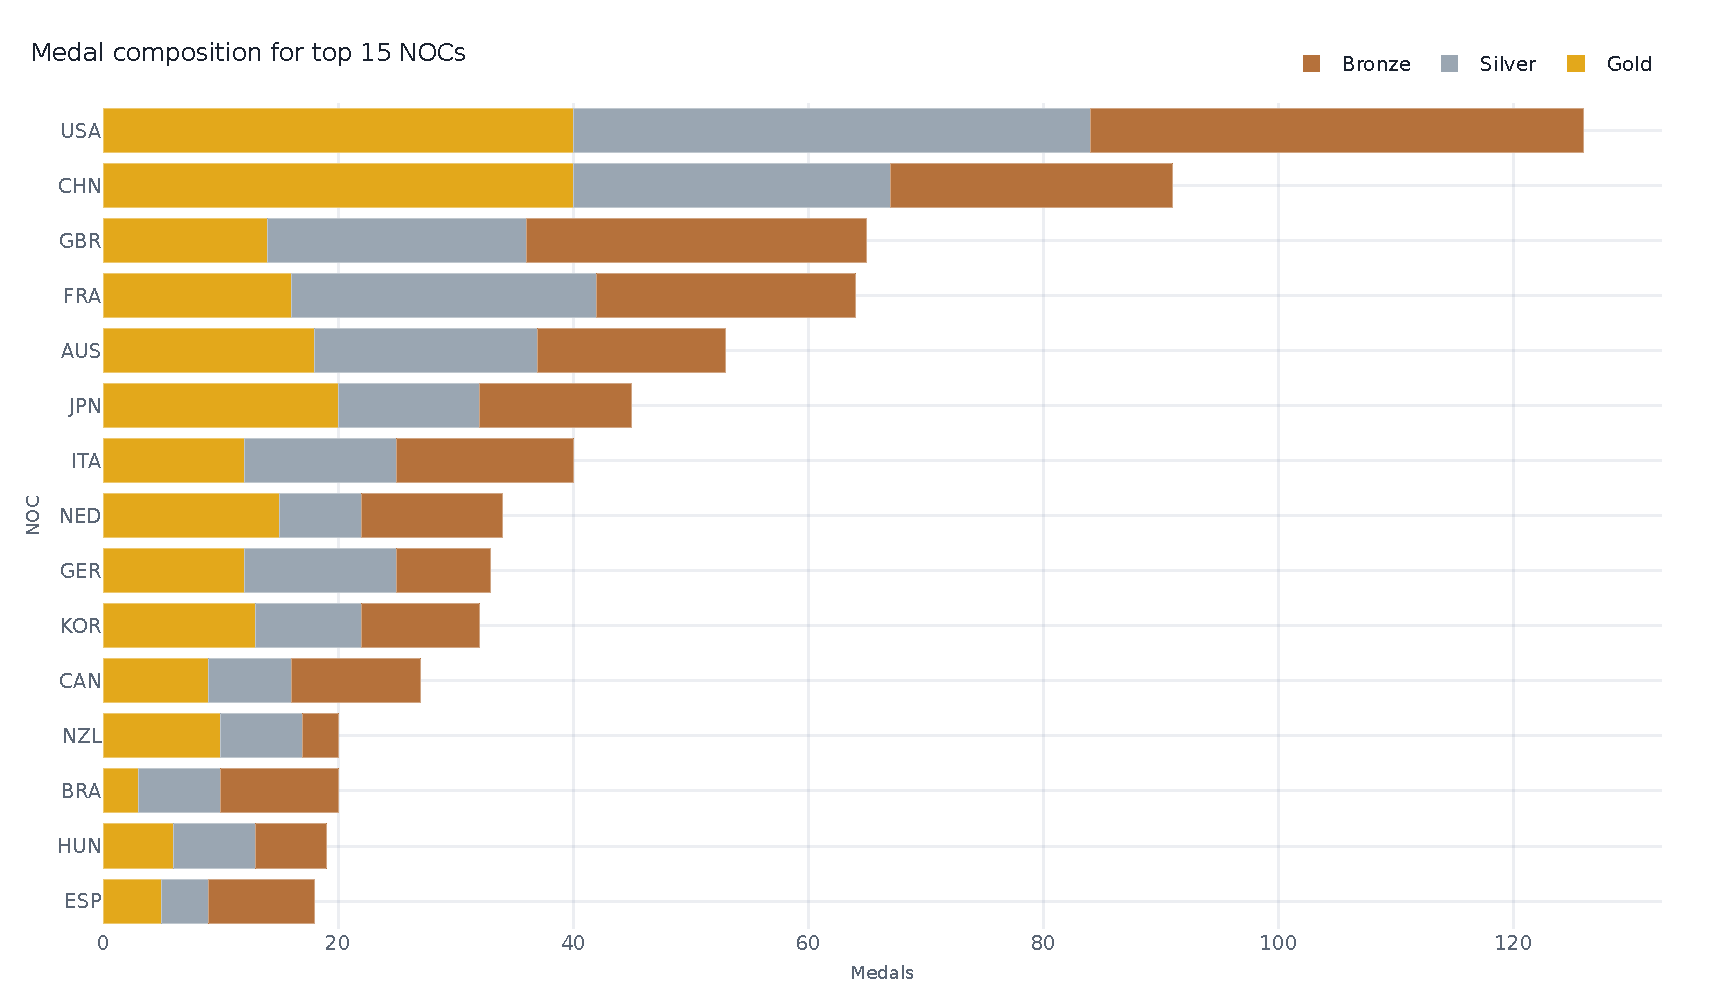
\includegraphics[width=0.49\linewidth]{figures/medal_composition.pdf}\hfill
  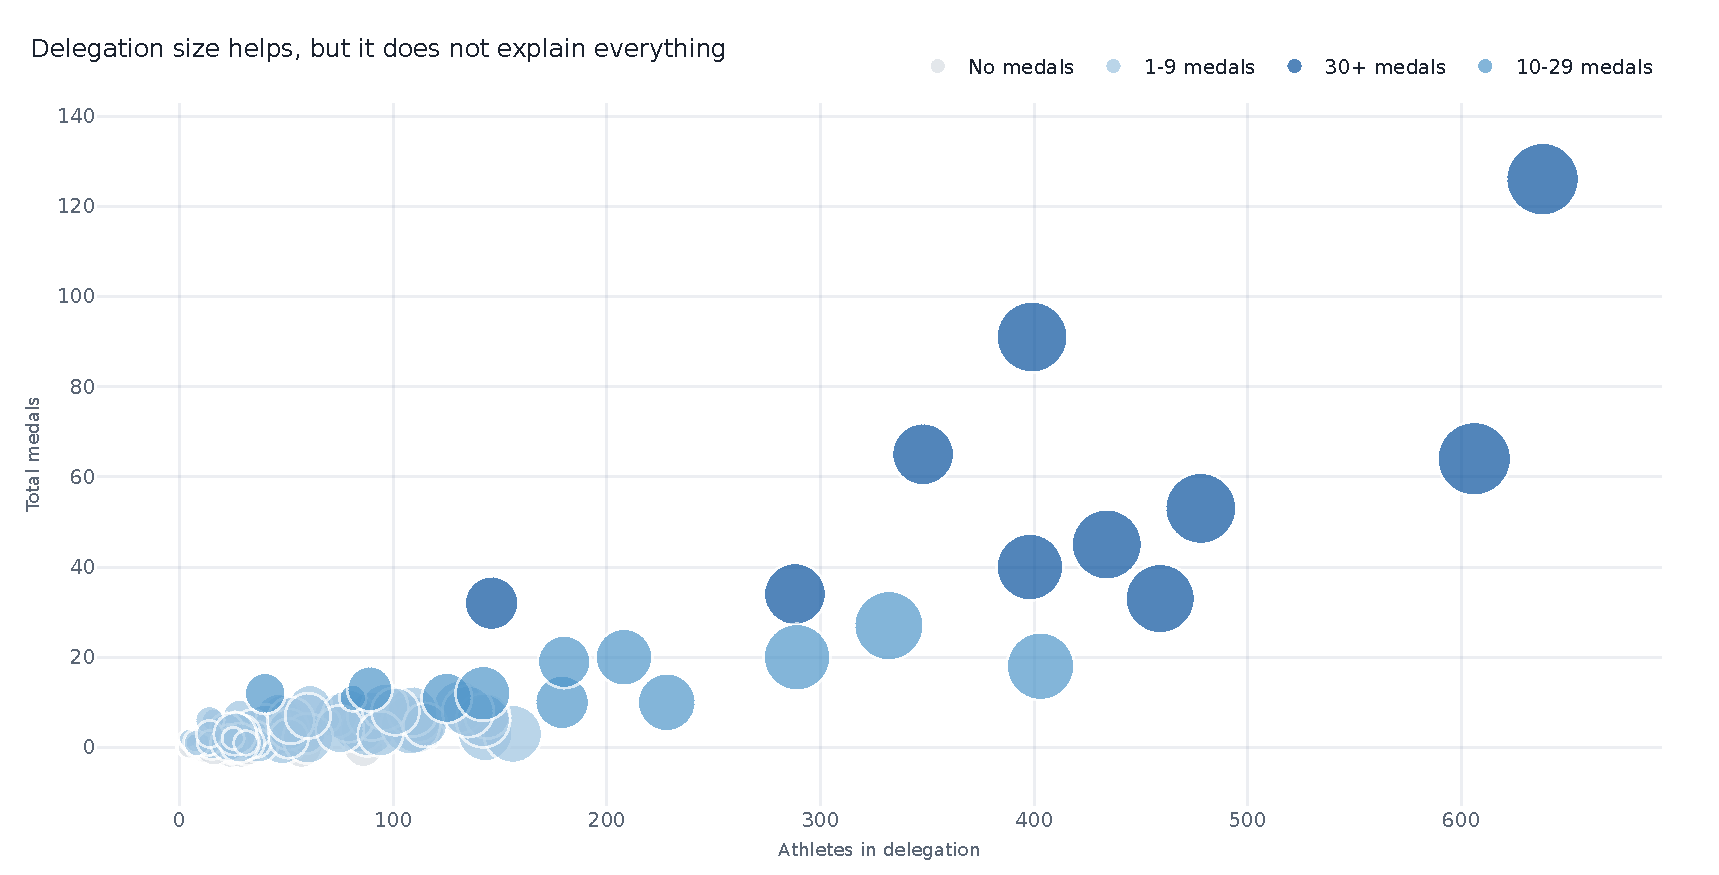
\includegraphics[width=0.49\linewidth]{figures/athletes_vs_medals.pdf}
  \caption{\textbf{Encoding by data type.} Left: medal count as length, medal
  colour as hue. Right: a bubble scatter where position encodes two quantities,
  area a third, and an ordered colour ramp the medal tier. Delegation size helps
  but does not fully explain medal output.}
  \label{fig:stack}
\end{figure}

\noindent To make the encoding discipline auditable at a glance, Table~\ref{tab:rationale}
maps \emph{every} chart in the dashboard to its variables (with measurement
levels), the marks and channels it uses, and the design principle behind the
choice. The recurring pattern is deliberate: quantities go to position and length
(the most accurately decoded channels), categories to hue, and area is used only
where a hierarchy or a third variable justifies it --- always with labels, because
area is systematically underestimated.

{\footnotesize\sffamily
\renewcommand{\arraystretch}{1.25}
\rowcolors{2}{softgray}{white}
\begin{longtable}{@{}p{0.155\linewidth} p{0.245\linewidth} p{0.20\linewidth} p{0.30\linewidth}@{}}
\caption{Per-chart encoding rationale. Type codes: N nominal, O ordinal, Q
quantitative, T temporal, S spatial.}\label{tab:rationale}\\
\toprule
\rowcolor{charcoal}\textbf{\color{white}Chart (tab)} & \textbf{\color{white}Variables (type)} & \textbf{\color{white}Marks \& channels} & \textbf{\color{white}Encoding rationale} \\
\midrule
\endfirsthead
\rowcolor{charcoal}\textbf{\color{white}Chart (tab)} & \textbf{\color{white}Variables (type)} & \textbf{\color{white}Marks \& channels} & \textbf{\color{white}Encoding rationale} \\
\midrule
\endhead
\midrule \multicolumn{4}{r}{\footnotesize\emph{continued on next page}}\\
\endfoot
\bottomrule
\endlastfoot
World choropleth \emph{(Opening Lens)} & NOC (N), total medals (Q), country geometry (S) & Region fill; colour \emph{value} & Spatial magnitude by region; value encodes order (Bertin); leaders separate pre-attentively. \\
Medal composition \emph{(Medal Race)} & NOC (N), count (Q), medal type (O) & Bar \emph{length}; hue per tier & Length is the most accurate channel for quantity (Cleveland\,--\,McGill); fixed hue order survives grayscale. \\
Athletes vs.\ medals \emph{(Opening Lens)} & Athletes (Q), medals (Q), disciplines (Q), tier (O) & x/y \emph{position}; area; colour value & Position for the two key quantities; area and value carry secondary variables in one exploratory view. \\
Specialization heatmap \emph{(Specialization)} & NOC (N), discipline (N), records (Q) & Cell colour value + printed text & Pre-attentive detection of hot cells; redundant text gives exact magnitude (multiple encodings). \\
Medal-flow Sankey \emph{(Specialization)} & NOC (N), discipline (N), colour (N), flow (Q) & Nodes + ribbon \emph{width} & $k$-partite flow graph; ribbon width encodes the weighted edge (flow volume). \\
Treemap \emph{(Specialization)} & Discipline (N), country (N), records (Q) & Nested \emph{area} + colour value & Hierarchy with proportional ink; tile labels offset the lower accuracy of area. \\
Age distribution \emph{(Athlete Lens)} & Age (Q), gender (N) & Bar length (freq.); hue & Distribution shape on a zero baseline; gender overlaid for direct comparison. \\
Gender balance \emph{(Athlete Lens)} & Discipline (N), gender (N), share (Q) & Bar length (share); hue & 100\,\% stacked: reads part-to-whole \emph{share}, not raw counts. \\
Age by discipline \emph{(Athlete Lens)} & Discipline (N), age (Q) & Box glyph; position (quartiles) & Distribution by group; shows spread without implying sampling error. \\
Competition load \emph{(Athlete Lens)} & Events (Q), active days (Q), medals (Q), status (N) & x/y position; area; hue & Three-variable relationship; capped bubble size + sampling manage overlap. \\
Medal efficiency \emph{(Medal Race)} & NOC (N), medals per 100 athletes (Q, ratio) & Bar length & A normalized rate --- the honest per-athlete complement to the absolute-count map. \\
Tokyo delta \emph{(Medal Race)} & NOC (N), medal change (Q, signed) & Bar length; diverging hue + label & Change around a zero centre; a labelled direction is a second, non-colour cue (CVD-safe). \\
Venue symbol map \emph{(Geography)} & Venue (N), lat/long (S), athletes (Q), medal activity (Q) & Map position; size; colour & Point/symbol map; size and colour ride on top of geographic position. \\
Daily medals \emph{(Medal Race)} & Games day (T), colour (N), count (Q) & x\,=\,time; bar length; hue & Trend over time; the static frame of the animated cumulative race. \\
Competition timeline \emph{(Geography)} & Start date (T), athletes (Q), medalists (Q) & x\,=\,time; bar length + line & Temporal rhythm on a single honest count axis --- no dual axis. \\
Records by discipline \emph{(Geography)} & Discipline (N), records (Q) & Bar length & Amounts, ranked --- the simplest accurate encoding for a count. \\
\end{longtable}
}

% ---------- Chapter 3 ----------
\subsection{Graphical perception}
\applied
\begin{techbox}
Signal detection and Weber's law / JND; magnitude estimation ---
Stevens' power law~\cite{stevens1957}, by which \emph{area is underestimated} while
length is near-unbiased, and the Cleveland \& McGill (1984) accuracy
ordering~\cite{cleveland1984} (position\,$>$\,length\,$>$\,angle\,$>$\,area), as
summarized by Munzner~\cite{munzner2014}; pre-attentive processing;
multiple encodings; Gestalt grouping; and change blindness.
\end{techbox}
\howapplied
The country$\times$discipline heatmap (Fig.~\ref{fig:heat}) uses colour intensity
so concentrations (USA swimming, Netherlands hockey, GBR rowing) are detected
\textbf{pre-attentively}, while printed cell values give exact magnitudes where
colour is imprecise. Magnitude comparisons use \textbf{bars} (length), never pie
angles --- the Cleveland \& McGill ordering --- and where a quantity is shown by
bubble \emph{area} (scatters, treemap) we cap size and label values, mindful that
area is systematically underestimated (Stevens' power law). The
Daily\,/\,Cumulative toggle and the animated race introduce a frame of motion;
pre-attentive colour guides the eye across it to limit \emph{change blindness}.
Gestalt \emph{similarity} (shared medal hues across pages) and \emph{proximity}
(paired two-column panels) bind related views.
\notesadj
Cell text is enabled on the heatmap precisely because colour intensity alone is
poor for reading exact counts --- a direct application of the
``multiple encodings'' principle.

\dashfig{specialization_heatmap.pdf}{0.98}{\textbf{Pre-attentive specialization.}
Medal-record counts by NOC and discipline. Dark cells (e.g.\ USA swimming~=70)
are spotted instantly; the overprinted numbers supply precise magnitudes.}{fig:heat}

% ---------- Chapter 4 ----------
\subsection{Charts for multivariate data}
\applied
\begin{techbox}
The standard chart families map one-to-one onto dashboard pages: amounts,
distributions, proportions, relationships, and trends/change. Coordinate systems
are Cartesian throughout; uncertainty is addressed below.
\end{techbox}
\howapplied
\begin{itemize}
  \item \textbf{Amounts:} discipline medal-record bars
        (Fig.~\ref{fig:amountpanel}, left) and the stacked medal-composition bar
        (Fig.~\ref{fig:stack}, left); the medal ranking is shown as a podium, not
        a table.
  \item \textbf{Distributions:} the age histogram by gender
        (Fig.~\ref{fig:distpanel}, left) and age box plots by discipline
        (Fig.~\ref{fig:agebox}).
  \item \textbf{Proportions:} the 100\,\% stacked gender-balance bar
        (Fig.~\ref{fig:distpanel}, right).
  \item \textbf{Relationships:} delegation size vs.\ medals
        (Fig.~\ref{fig:stack}, right), competition load
        (Fig.~\ref{fig:load}), and medal efficiency (Fig.~\ref{fig:eff}).
  \item \textbf{Trends / change:} the Paris-vs-Tokyo delta
        (Fig.~\ref{fig:amountpanel}, right), the day-by-day medal timeline
        (Fig.~\ref{fig:daily}), and the competition timeline
        (Fig.~\ref{fig:closepanel}, left).
\end{itemize}
\notesadj
\textbf{Uncertainty is intentionally not visualized.} The data are
\emph{complete event records}, not a sample with sampling error, so error bars
would imply a precision that does not exist; in line with best
practice~\cite{wilke2019}, we show full \emph{distributions} (box plots) rather
than lossy mean\,$\pm$\,error-bar summaries. \textbf{Trend smoothing} (LOESS,
moving averages) is likewise omitted: an Olympic calendar of $\sim$18 discrete
daily counts is too short for a meaningful smoother, so the day-by-day timeline
shows the raw counts. Coordinate systems are Cartesian throughout --- medal
totals are long-tailed, so a log axis was considered but rejected to keep the
zero-baseline bar reading intuitive for a general audience.

\begin{figure}[htbp]\centering
  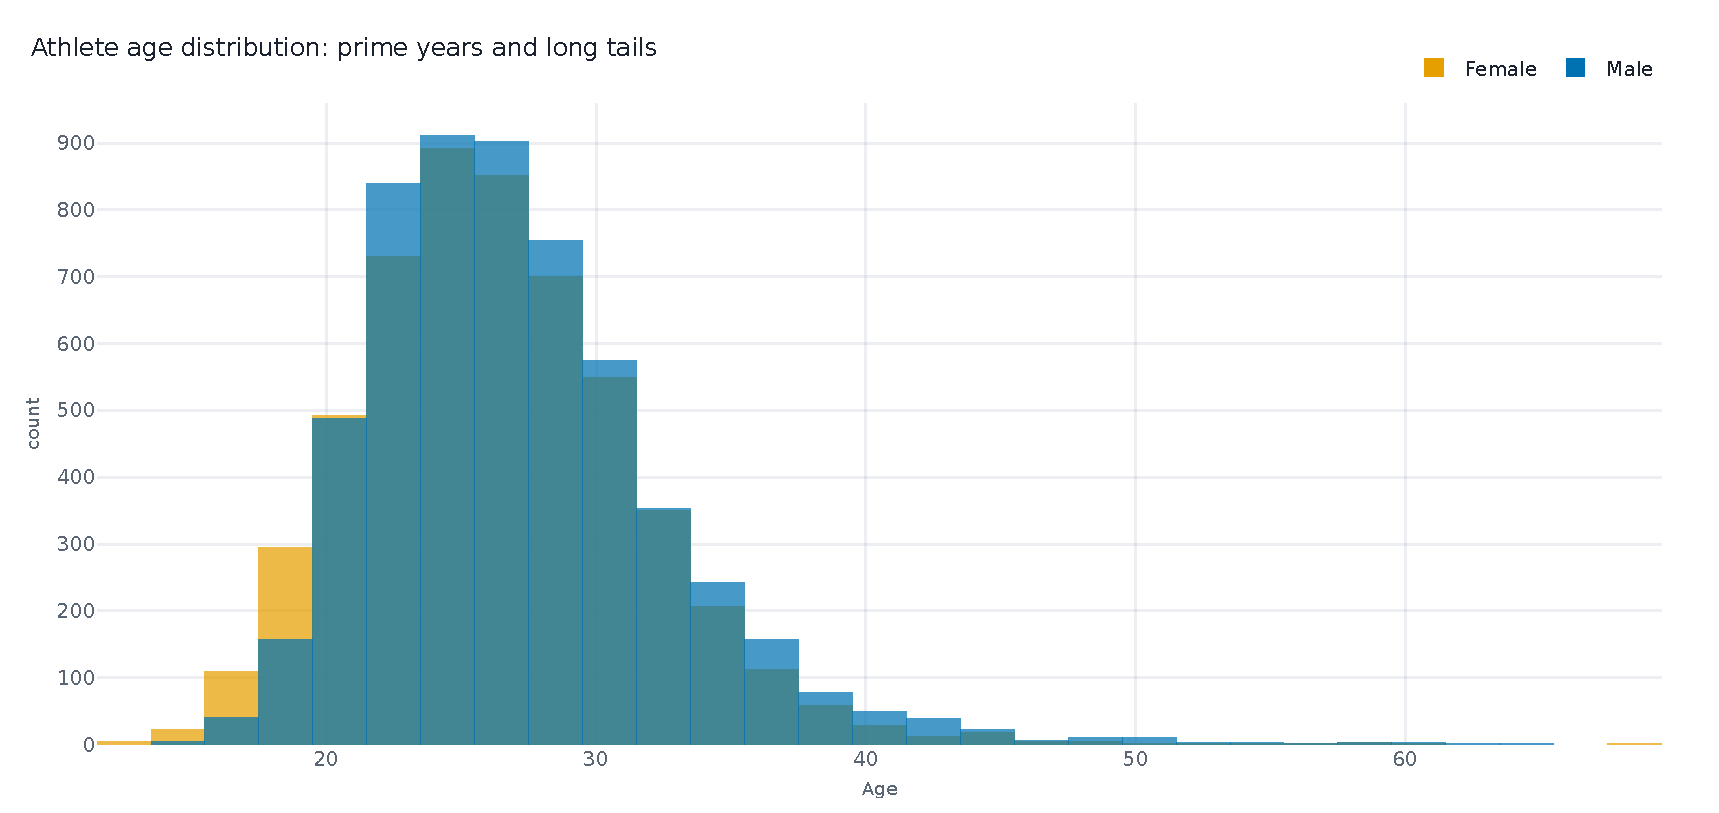
\includegraphics[width=0.49\linewidth]{figures/age_distribution.pdf}\hfill
  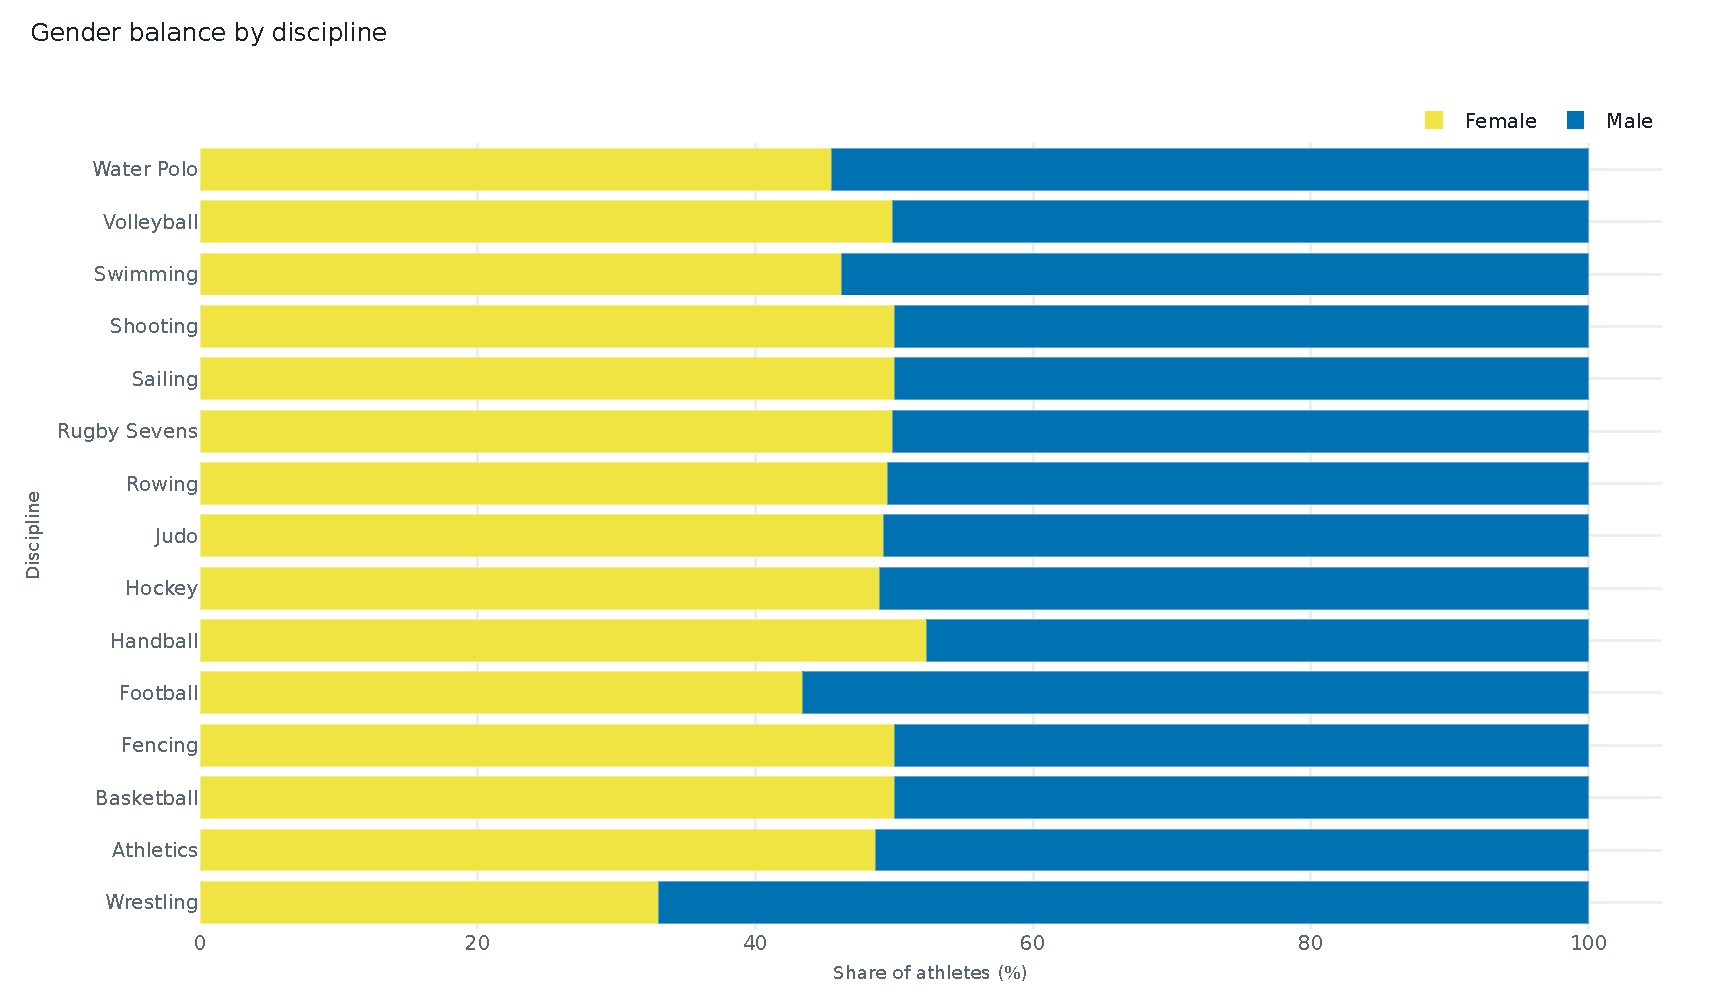
\includegraphics[width=0.49\linewidth]{figures/gender_balance.pdf}
  \caption{\textbf{Distributions and proportions.} Left: age distribution by
  gender, overlaid for direct comparison. Right: a 100\,\% stacked bar reading
  gender \emph{share} per discipline, not raw counts.}
  \label{fig:distpanel}
\end{figure}

\dashfig{age_by_discipline.pdf}{0.92}{\textbf{Distribution by group.} Age box
plots reveal sharply different sport profiles --- a median near 20 in
skateboarding and rhythmic gymnastics versus 39 in equestrian. Spread is shown
without implying sampling uncertainty.}{fig:agebox}

\begin{figure}[htbp]\centering
  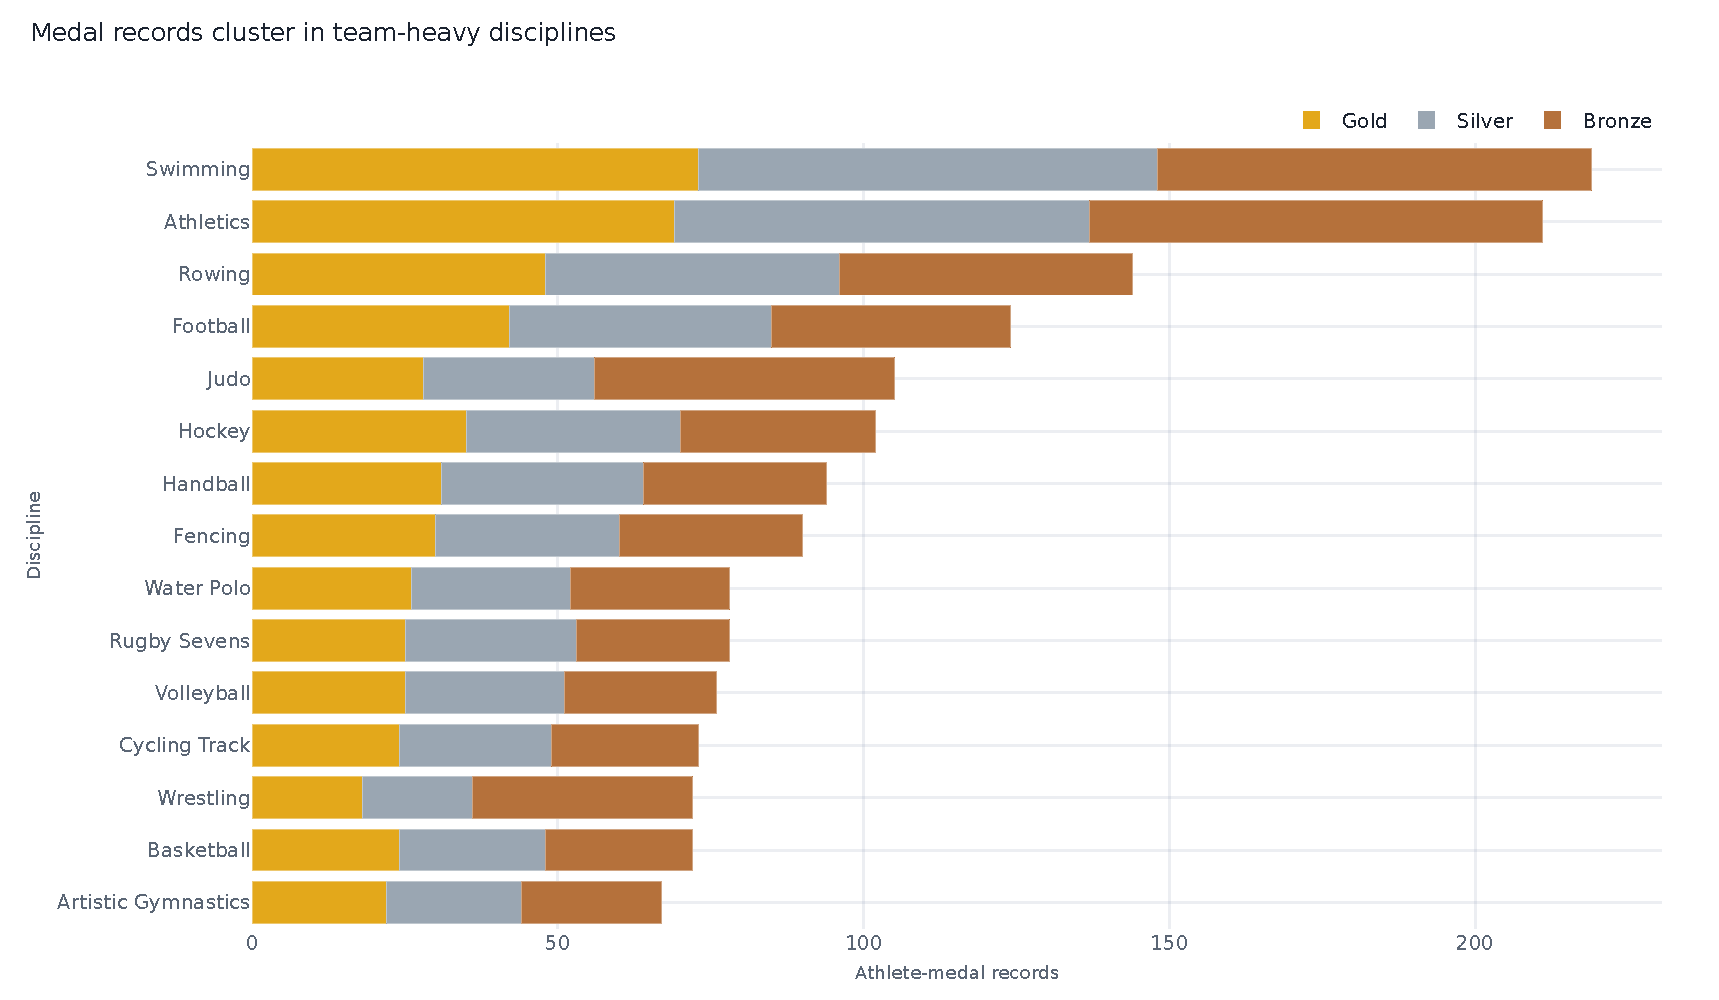
\includegraphics[width=0.49\linewidth]{figures/discipline_medals.pdf}\hfill
  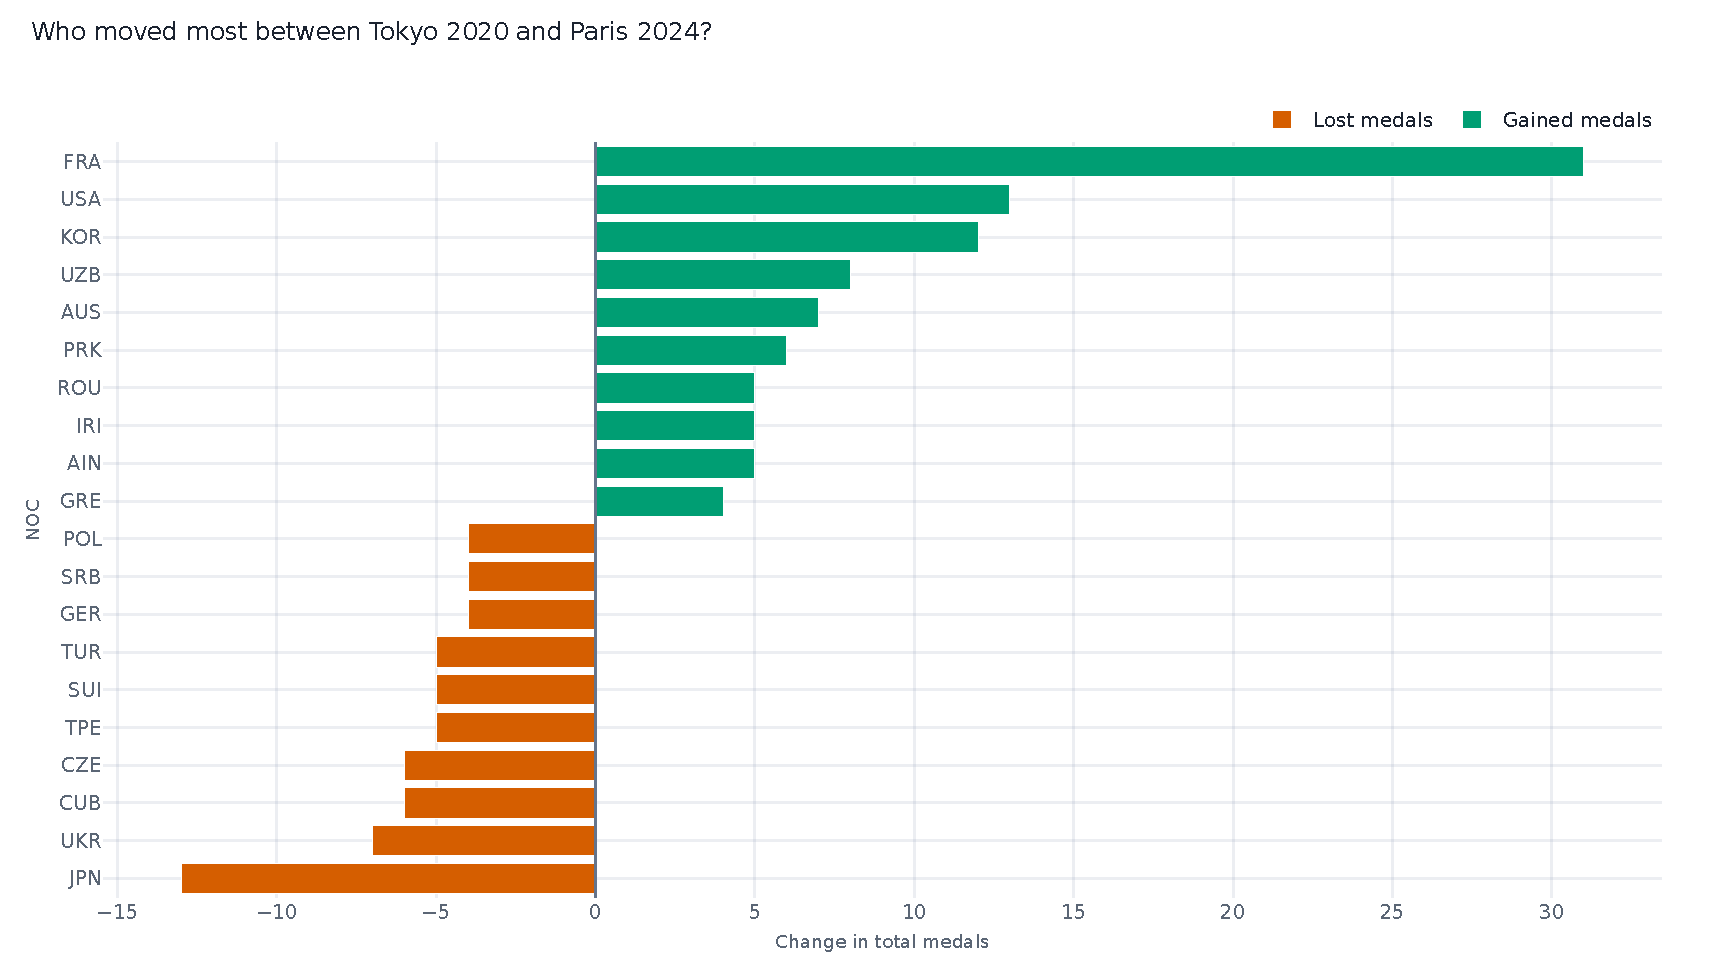
\includegraphics[width=0.49\linewidth]{figures/tokyo_delta.pdf}
  \caption{\textbf{Amounts and change.} Left: athlete--medal records per
  discipline, stacked by colour. Right: a diverging bar of the change in total
  medals from Tokyo to Paris --- France~+31, Japan~$-13$.}
  \label{fig:amountpanel}
\end{figure}

\dashfig{competition_load.pdf}{0.9}{\textbf{Relationship, three variables.}
Events entered vs.\ active competition days, with bubble area for medal count
and hue for medal status. Overlap is managed by capped bubble size and a
sampled draw (4{,}500 points) for dense regions.}{fig:load}

\dashfig{medal_efficiency.pdf}{0.82}{\textbf{Relationship, normalized.} Medals
per 100 athletes among delegations of $\geq$30 athletes --- the analytical
pay-off of the size-vs-medals scatter. It rewards small, sharp teams that the
raw medal table buries, and is the efficiency leaderboard shown in the Medal
Race tab.}{fig:eff}

% ---------- Chapter 5 ----------
\subsection{Graph and flow visualization}
\applied
\begin{techbox}
Graph data properties --- nodes, edges, \emph{directionality} and
\emph{edge weight} --- and graph visualization mechanisms. The
country$\rightarrow$discipline$\rightarrow$medal relationships form a directed,
weighted, three-layer graph --- \emph{$k$-partite}, generalising the
\emph{bipartite} graph --- rendered as a Sankey flow.
\end{techbox}
\howapplied
The medal-flow Sankey (Fig.~\ref{fig:sankey}) treats NOCs, disciplines, and
medal colours as three layers of \textbf{nodes}; \textbf{edge width} encodes the
number of athlete--medal records flowing along each path. The snap layout keeps
the three columns aligned so flow magnitude is read by ribbon thickness.
\notesadj
We are explicit that this is a \emph{derived categorical flow graph}, not an
athlete-to-athlete social network. Node-link layouts contrast with the
\emph{adjacency matrix}~\cite{munzner2014}; we choose a layered node-link/flow form
because this graph is \emph{dense by construction} (every co-occurring top NOC
$\times$ discipline) and the question is about \emph{flow volume}, which ribbon
width shows directly. A force-directed layout suits sparse connectivity networks,
not aggregated counts, and a matrix would hide the country$\rightarrow$medal path.
The Sankey thus extends standard flow-map and hierarchy (treemap) mechanisms.

\dashfig{medal_flow_sankey.pdf}{0.96}{\textbf{Derived flow graph.}
NOC~$\rightarrow$~discipline~$\rightarrow$~medal-colour flow. Ribbon width encodes
athlete--medal record volume; the three node columns are a $k$-partite graph
(a layered generalisation of the bipartite graph), not a connectivity network.}{fig:sankey}

% ---------- Chapter 6 ----------
\subsection{Figure design and graphical integrity}
\applied
\begin{techbox}
Proportional ink~\cite{bergstrom2016}, handling overlap, colour use and
accessibility, multi-panel figures, titles and captions, data--context balance,
table design, and avoiding 3D; plus the integrity rules of graphical honesty ---
the \emph{Lie Factor}, maximising the \emph{data--ink ratio}, and avoiding
\emph{chartjunk}~\cite{tufte2001}. The chart-choice and figure conventions follow
Wilke's \emph{Fundamentals of Data Visualization}~\cite{wilke2019}.
\end{techbox}
\howapplied
\begin{itemize}
  \item \textbf{Proportional ink:} every bar starts at zero; the treemap
        (Fig.~\ref{fig:treemap}) sizes rectangles strictly by record count.
  \item \textbf{Overlap:} the load scatter caps bubble size and samples dense
        regions; the heatmap replaces overplotted points with an aggregated grid.
  \item \textbf{Colour and accessibility:} the \emph{qualitative} palette is the
        \textbf{Okabe--Ito colourblind-safe} set~\cite{okabeito2008}, reused across pages; the
        \emph{sequential} map, heatmap, and treemap scales are perceptually
        ordered single-hue / Viridis ramps (not Okabe--Ito, which is categorical);
        medal hues stay constant and luminance-distinct (so they survive grayscale).
        Where a category is carried by colour alone (medal tier, medal status,
        gender) the palette is CVD-safe and the legend and tooltip disambiguate;
        gain/loss adds a second, non-colour cue --- a labelled direction --- and
        status charts colour only the ``achieved'' series, leaving the rest neutral
        gray (context ink).
  \item \textbf{Graphical integrity (Lie Factor $\approx$ 1):} every bar starts at
        zero, no axis is truncated, there are no dual axes, and no one-dimensional
        quantity is encoded as a two-dimensional radius --- so the chart cannot
        overstate an effect. The restrained, KPI-led layout maximises the
        \emph{data--ink ratio} and avoids \emph{chartjunk} (the podium is the one
        deliberately ``useful'' embellishment).
  \item \textbf{Multi-panel:} two-column panels (e.g.\ Figs.~\ref{fig:stack},
        \ref{fig:distpanel}) place complementary views side by side.
  \item \textbf{Titles \& captions:} chart titles state a finding
        (``Delegation size helps, but it does not explain everything''), not just
        the variables.
  \item \textbf{Tables, when used, follow the six rules:} good practice is both to
        ``replace a table with a chart'' \emph{and} to set any remaining table
        well~\cite{wilke2019}, so the dashboard prefers charts (values live on
        hover, no raw grids), but where
        this \emph{report} does tabulate (e.g.\ Tables~\ref{tab:files},
        \ref{tab:datatypes}, \ref{tab:rationale}) it obeys Wilke's six guidelines:
        no vertical rules, horizontal rules only at the header and boundaries,
        text columns left-aligned, and number columns right-aligned to equal
        precision.
  \item \textbf{No 3D:} every chart is 2D; depth is never used decoratively.
\end{itemize}
\notesadj
The treemap is the one area-encoded chart; because area is harder to compare than
length, it is used only for \emph{hierarchy} (discipline$\rightarrow$country),
with exact values labelled on each tile.

\dashfig{medal_treemap.pdf}{0.9}{\textbf{Hierarchy with proportional ink.}
Medal records nested discipline~$\rightarrow$~country. Tile area is strictly
proportional to count and colour reinforces the same magnitude (darker = more
records); labels supply exact values to offset the lower accuracy of area
judgements.}{fig:treemap}

% ---------- Chapter 7 ----------
\subsection{Map visualization}
\applied
\begin{techbox}
Map foundations and map types: a \textbf{choropleth} for region-level intensity
and a \textbf{symbol (bubble) map} for point locations, each with its own
projection and geocoding concerns.
\end{techbox}
\howapplied
The world choropleth (Fig.~\ref{fig:map}) encodes total medals as fill intensity
on a Natural Earth projection, after mapping Olympic NOC codes to standard ISO-3
country codes. The venue bubble map (Fig.~\ref{fig:venue}) places venues by
latitude/longitude on a Carto base layer, with \textbf{bubble size} for athlete
volume and \textbf{colour} for medal activity --- showing how the Games spread
from a dense Paris cluster to outlying and overseas venues.
\notesadj
The choropleth encodes \emph{absolute} medal totals, which visually over-weights
large delegations --- a known limitation of choropleths that cartograms address. The
honest complement is a per-athlete \emph{rate}, which we provide as the
medals-per-100-athletes efficiency bar (Fig.~\ref{fig:eff}) rather than a second
map, since no population data is in scope for a true per-capita choropleth. The
venue map's Carto base is Web-Mercator, whose distortion is negligible at France's
latitude. Records without coordinates (``multisite'' rows) are excluded from map
layers but retained everywhere else (\S\ref{sub:concept}); the choropleth omits
mixed teams (AIN, EOR) that have no country geometry.

\dashfig{venue_geography.pdf}{0.96}{\textbf{Symbol map.} Paris~2024 venues across
France. Bubble size encodes athlete volume, colour encodes total athlete medals;
the dense Paris cluster contrasts with sailing/surf venues far to the south.}{fig:venue}

% ---------- Chapter 8 ----------
\subsection{Interaction}
\applied
\begin{techbox}
Interaction techniques --- filtering, zoom, and view transformation ---
together with \emph{animation}, details-on-demand, and the tools used.
\end{techbox}
\howapplied
Interaction is \textbf{inline and direct} --- no sidebar. Controls live in the
page next to the charts they affect: \textbf{filtering} via segmented-control
pills (gender, medal status, medal colours) and multiselects (focus NOCs,
disciplines), and \textbf{view transformation} via top-$N$ sliders, an age-range
slider, a medal-sort selector that re-ranks charts live, and a Daily\,/\,Cumulative
toggle on the medal timeline (Fig.~\ref{fig:daily}). The five sections are
switched with \textbf{tabs}. Every chart adds \textbf{details-on-demand}
via hover tooltips and \textbf{zoom/pan} via the chart toolbar; the maps support
drag-pan and scroll-zoom. Each section owns the controls relevant to it, so a
reader explores one question at a time. Table~\ref{tab:interaction} maps each
interaction to the control that exposes it and the analytical task it serves.

\begin{table}[htbp]
\centering\small\sffamily
\renewcommand{\arraystretch}{1.2}
\rowcolors{2}{softgray}{white}
\begin{tabularx}{\linewidth}{l l X}
\toprule
\rowcolor{charcoal}\textbf{\color{white}Interaction} & \textbf{\color{white}Control (where)} & \textbf{\color{white}Analytical task it serves} \\
\midrule
Navigate views   & Top tabs               & Switch between the five story acts (no sidebar). \\
Filter           & Segmented pills        & Subset by gender, medal status, or medal colour. \\
Filter           & Multiselects           & Compare a chosen set of NOCs or disciplines. \\
View transform   & Top-$N$ slider         & Focus on the leaders and cut clutter. \\
Filter           & Age-range slider       & Restrict to a demographic sub-population. \\
Re-order         & Medal-sort selector    & Re-rank charts live by the chosen metric. \\
View transform   & Daily\,/\,Cumulative toggle & Switch the medal timeline's representation. \\
Animation        & Race ``play'' button   & Watch cumulative medals build over the Games. \\
Details-on-demand& Hover tooltip          & Read exact values where a channel is imprecise. \\
View transform   & Zoom / pan             & Inspect dense regions of a map or chart. \\
Filter           & Legend toggle          & Show or hide an individual series. \\
\bottomrule
\end{tabularx}
\caption{Interaction-to-task mapping. Every control is inline, beside the chart it
drives, so each interaction answers a specific analytical question.}
\label{tab:interaction}
\end{table}

\textbf{Animation.} The Medal Race tab adds an animated bar-chart race:
pressing \emph{play} steps through the Games day by day while each discipline's
bar grows with its cumulative medal haul. Animation is used \emph{here and only
here} because the encoded variable --- cumulative medals --- is genuinely
time-ordered, so motion carries information rather than decoration. A static
companion view (Fig.~\ref{fig:daily}) shows the same rhythm as daily stacked bars
for readers who prefer one frame.
\notesadj
We deliberately restrict animation to the one time-ordered variable; the rest of
the dashboard is a completed-event snapshot where interactive filtering is the
more analytical form of dynamics. Every filtered view is verified to degrade to a
styled ``no data'' placeholder rather
than crash on an empty selection.

\dashfig{daily_medals.pdf}{0.96}{\textbf{Trend over time.}
Athlete-medals awarded per Games day, stacked by colour --- the static frame of
the animated medal race. The tally builds slowly, dips mid-Games, then surges
across the closing weekend, peaking on 10 August.}{fig:daily}

% ---------- Chapter 9 ----------
\subsection{Storytelling and narrative}
\applied
\begin{techbox}
Fundamental principles~\cite{knaflic2015} --- the three pillars (\emph{data},
\emph{visualisation}, \emph{narrative}), \emph{understand the context} (audience and
purpose), and the three-act \emph{story structure}
hook\,$\rightarrow$\,analysis\,$\rightarrow$\,resolution; storytelling techniques
--- simple-text headline numbers, takeaway titles, redundant encoding;
\emph{narrative style} --- author-driven vs reader-driven; and interaction and
exploration within the story.
\end{techbox}
\howapplied
\textbf{Understand the context.} Before any chart, we fixed the audience and the
message. The audience is a \emph{general, data-literate} classroom, not domain
analysts; the single \emph{main message} is that ``\emph{the medal table hides
most of what made Paris~2024 interesting},'' and the purpose is to make that case
visually and then hand the data over for exploration. Every design choice
(headline numbers first, no raw tables, one takeaway per chart) follows from that
audience and that message.

\textbf{Story structure.} Each tab is a three-act beat --- a \emph{hook} (a
one-line guiding question such as ``Who led Paris~2024, and who changed most since
Tokyo?''), an \emph{analysis} that builds the answer in charts, and a
\emph{resolution} in the takeaway title and a spotlight. Across tabs the arc moves
\emph{macro-to-micro}, from global geography to the individual athlete and venue,
so abstract totals become concrete and human; the closing timeline and record bar
(Fig.~\ref{fig:closepanel}) end the Games on their daily rhythm.

\textbf{Narrative style.} The story is \textbf{author-driven} in its fixed tab
order and messaged titles, but becomes \textbf{reader-driven} on each page, where
filters and tooltips let the reader test their own hypotheses. The Paris-vs-Tokyo
delta is a \emph{before/after} contrast, and the five linked tabs are
\emph{progressive disclosure} --- multiple charts revealing one facet at a time
(Bach et al.\ 2017~\cite{bach2017}) rather than one over-loaded view.
\notesadj
We apply the standard storytelling devices: \textbf{simple text} (one prominent
number with a few supporting words, shown as the KPI cards), \textbf{takeaway
titles} that state the finding rather than the variables (the good-vs-bad-title
contrast~\cite{knaflic2015}), and \textbf{redundant encoding} (data labels and
annotations alongside colour). We also heed the ``\emph{same data, different
stories}'' caution on storytelling as a double-edged tool: every chart labels its
unit (athlete-medals vs official medals) so the framing persuades without
misleading. The ``executive-overview-first'' layout, the podium, and the
host-nation (France) spotlight are additionally informed by \emph{The Big Book of
Dashboards}~\cite{bigbook2017}; we \textbf{replaced every raw data table with a
visual}, keeping detail on demand in tooltips --- a dashboard should show the
data, not dump it.

\begin{figure}[htbp]\centering
  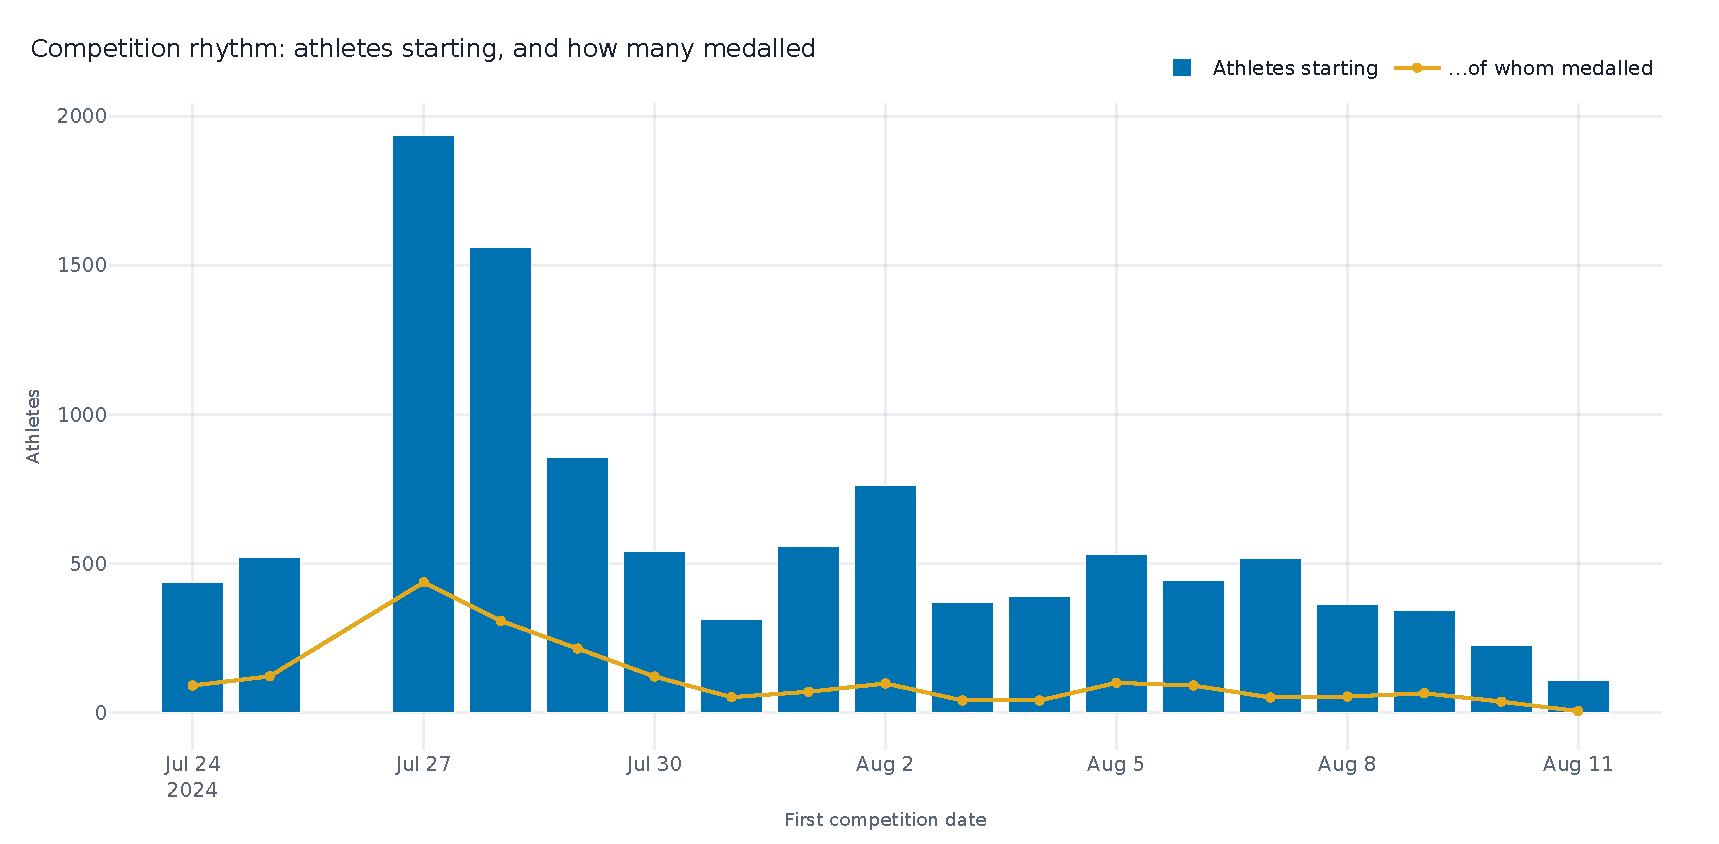
\includegraphics[width=0.49\linewidth]{figures/competition_timeline.pdf}\hfill
  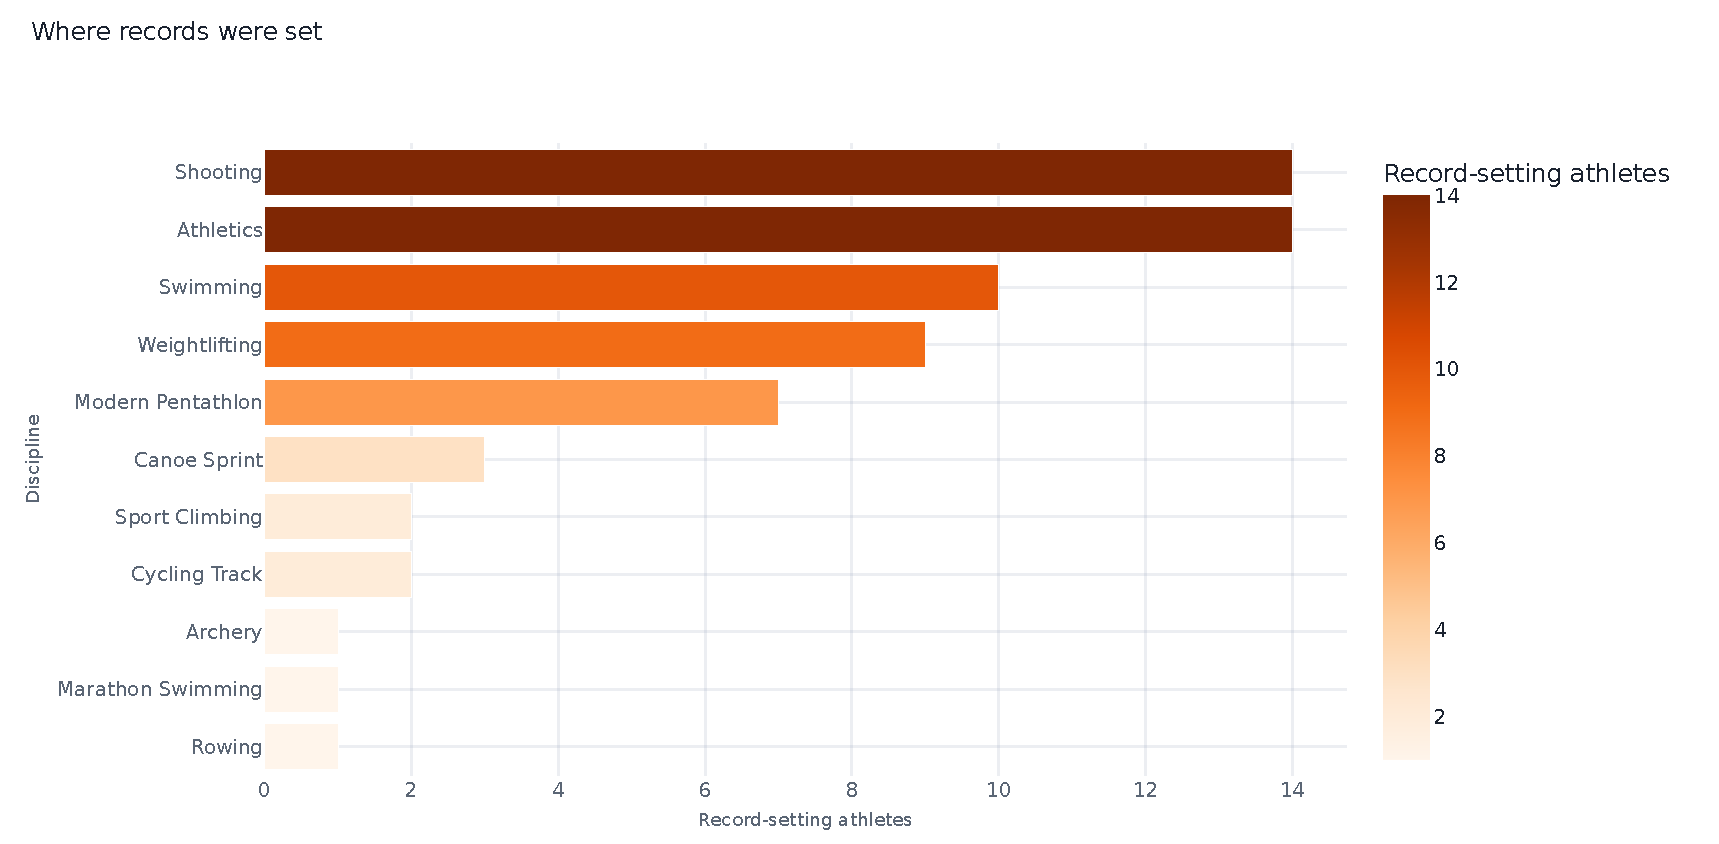
\includegraphics[width=0.49\linewidth]{figures/records_by_discipline.pdf}
  \caption{\textbf{Closing the story.} Left: competition rhythm by athletes'
  first-start date --- bars are athletes starting, the gold line the subset who
  medalled, both on one honest count axis. Right: where the 64 records were set.}
  \label{fig:closepanel}
\end{figure}

% ===================== 6. INSIGHTS ==================================
\section{Key Insights}
\label{sec:insights}

\begin{insightbox}{1. The gold race was a dead heat; the medal race was not.}
The United States and China each won \textbf{40 golds}, but the United States
took \textbf{126 total medals to China's 91}, driven by depth across many
disciplines rather than a few dominant sports (visible in the choropleth and
heatmap).
\end{insightbox}
\begin{insightbox}{2. Hosting moved the table.}
France gained \textbf{+31} medals versus Tokyo (33$\rightarrow$64), the largest
swing of any NOC, while \textbf{Japan fell $-13$} (58$\rightarrow$45). The
diverging delta chart makes the host effect legible at a glance.
\end{insightbox}
\begin{insightbox}{3. Specialization, not breadth, defines mid-tier powers.}
The heatmap shows concentrated strengths --- Netherlands in hockey, Great Britain
in rowing, Australia in swimming --- whereas the top two NOCs spread medals
broadly.
\end{insightbox}
\begin{insightbox}{4. The field reached near gender parity, with sport-specific age profiles.}
Women made up \textbf{49.1\,\%} of athletes; the median athlete was \textbf{26},
but discipline medians ranged from \textbf{20} (skateboarding, rhythmic
gymnastics) to \textbf{39} (equestrian) --- a spread the box plots surface
immediately.
\end{insightbox}
\begin{insightbox}{5. The Games were geographically dispersed.}
Although venues cluster in Paris, the symbol map shows competition reaching far
south (sailing in Marseille, plus overseas surfing), reinforcing that Paris~2024
was a spatial event, not a single-city one.
\end{insightbox}

% ===================== 7. CONCLUSION ================================
\section{Conclusion and Future Work}
\label{sec:conclusion}

The project set out to show that \emph{a flat medal table hides most of what made
Paris~2024 interesting}, and the dashboard makes that case visually: the global
choropleth, the Tokyo delta, the specialization heatmap, the athlete
distributions, and the venue map each surface a facet --- depth, host effect,
specialization, demographics, dispersion --- that a ranked table cannot. Just as
importantly, the build is a deliberate exercise in technique: every chart's
encoding is chosen by data type and justified against established criteria
(Table~\ref{tab:rationale}), colour is the Okabe--Ito colourblind-safe set used
only to carry meaning, the figures keep a Lie Factor of about one, and the
five-act arc applies recognized storytelling principles~\cite{knaflic2015}.

We are deliberate about the limits. The dashboard reports \emph{complete event
records}, not a sample, so it shows full distributions rather than error bars; the
choropleth encodes \emph{absolute} medal totals, with the medals-per-100-athletes
bar standing in for the per-capita rate a cartogram would otherwise provide; and
athlete height is too sparse (54\,\% missing) to be a core metric. Natural next
steps follow directly: bring in national-population data for a true per-capita
choropleth or cartogram; add a live data-refresh path so the same pipeline serves
future Games; run a short colour-blindness and usability check with real users;
and, where future data carries genuine sampling, add the uncertainty layer we
currently and correctly omit.

% ===================== 8. REPRODUCIBILITY ===========================
\section{Reproducibility}
\label{sec:repro}

Every figure in this report is generated directly from the same code and the same
prepared data that produce the live dashboard --- there are no screenshots and no
separately drawn figures --- and the document is typeset from those vector outputs.
Each figure shown here is therefore identical to what a reader sees in the
application, and the report cannot drift out of step with the dashboard.

The dashboard was exercised systematically across all five sections and every
interactive control, including empty and narrowly filtered selections; each of
these degrades gracefully to a styled ``no data'' state rather than failing. The
row counts, data types, and missing-value rates reported in \S\ref{sec:cleaning}
were checked against the underlying data and reconcile exactly. Together these
checks make the figures trustworthy: they are reproducible from the source data
and consistent with the application that produced them.

\vspace{0.6cm}
\noindent\rule{\linewidth}{0.4pt}\\[2pt]
{\footnotesize\sffamily\color{slate}
Data: Paris~2024 public CSVs (paris2024-data, GitHub) and the data.gouv.fr
enriched athlete table (ODbL). Built with Streamlit and Plotly; figures are
generated directly from the dashboard's own charting code.}

% ===================== REFERENCES ===================================
\addcontentsline{toc}{section}{References}
\begingroup
\small
\begin{thebibliography}{99}
\bibitem{bertin1983} J.~Bertin. \emph{Semiology of Graphics: Diagrams, Networks, Maps}. University of Wisconsin Press, 1983 (orig.\ 1967).
\bibitem{mackinlay1986} J.~Mackinlay. Automating the design of graphical presentations of relational information. \emph{ACM Transactions on Graphics}, 5(2):110--141, 1986.
\bibitem{cleveland1984} W.~S.~Cleveland and R.~McGill. Graphical perception: theory, experimentation, and application to the development of graphical methods. \emph{Journal of the American Statistical Association}, 79(387):531--554, 1984.
\bibitem{card1999} S.~K.~Card, J.~D.~Mackinlay, and B.~Shneiderman. \emph{Readings in Information Visualization: Using Vision to Think}. Morgan Kaufmann, 1999.
\bibitem{munzner2014} T.~Munzner. \emph{Visualization Analysis and Design}. CRC Press, 2014.
\bibitem{stevens1957} S.~S.~Stevens. On the psychophysical law. \emph{Psychological Review}, 64(3):153--181, 1957.
\bibitem{tufte2001} E.~R.~Tufte. \emph{The Visual Display of Quantitative Information}, 2nd ed. Graphics Press, 2001.
\bibitem{bergstrom2016} C.~T.~Bergstrom and J.~D.~West. The principle of proportional ink. 2016. \url{https://callingbullshit.org}.
\bibitem{wilke2019} C.~O.~Wilke. \emph{Fundamentals of Data Visualization}. O'Reilly Media, 2019.
\bibitem{knaflic2015} C.~N.~Knaflic. \emph{Storytelling with Data: A Data Visualization Guide for Business Professionals}. Wiley, 2015.
\bibitem{okabeito2008} M.~Okabe and K.~Ito. Color universal design (CUD): how to make figures and presentations friendly to colourblind people. 2008.
\bibitem{bach2017} B.~Bach, N.~Henry-Riche, S.~Carpendale, et al. Narrative design patterns for data-driven storytelling. In \emph{Data-Driven Storytelling}. CRC Press, 2017.
\bibitem{bigbook2017} S.~Wexler, J.~Shaffer, and A.~Cotgreave. \emph{The Big Book of Dashboards}. Wiley, 2017.
\bibitem{paris2024data} taniki. \emph{paris2024-data}. GitHub. \url{https://github.com/taniki/paris2024-data}.
\bibitem{datagouv} data.gouv.fr. \emph{Les athletes des Jeux Olympiques de Paris 2024} (ODbL). \url{https://www.data.gouv.fr/datasets/les-athletes-des-jeux-olympiques-de-paris-2024}.
\end{thebibliography}
\endgroup

\end{document}
